%%%%%%%%%%%%%%%%%%%%%%%%%%%%%%%%%%%%%%%%%
% Beamer Presentation
% LaTeX Template
% Version 1.0 (10/11/12)
%
% This template has been downloaded from:
% http://www.LaTeXTemplates.com
%
% License:
% CC BY-NC-SA 3.0 (http://creativecommons.org/licenses/by-nc-sa/3.0/)
%
%%%%%%%%%%%%%%%%%%%%%%%%%%%%%%%%%%%%%%%%%

%----------------------------------------------------------------------------------------
%	PACKAGES AND THEMES
%----------------------------------------------------------------------------------------

\documentclass[UTF8,aspectratio=169,14pt]{ctexbeamer}

\usepackage{hyperref}
\hypersetup{
	colorlinks=true,
	linkcolor=red,
	anchorcolor=blue,
	citecolor=green
}

\mode<presentation> {
	
	% The Beamer class comes with a number of default slide themes
	% which change the colors and layouts of slides. Below this is a list
	% of all the themes, uncomment each in turn to see what they look like.
	
	%\usetheme{default}
	%\usetheme{AnnArbor}
	%\usetheme{Antibes}
	%\usetheme{Bergen}
	%\usetheme{Berkeley}
	%\usetheme{Berlin}
	%\usetheme{Boadilla}
	%\usetheme{CambridgeUS}
	%\usetheme{Copenhagen}
	%\usetheme{Darmstadt}
	%\usetheme{Dresden}
	%\usetheme{Frankfurt}
	%\usetheme{Goettingen}
	%\usetheme{Hannover}
	%\usetheme{Ilmenau}
	%\usetheme{JuanLesPins}
	%\usetheme{Luebeck}
	\usetheme{Madrid}
	%\usetheme{Malmoe}
	%\usetheme{Marburg}
	%\usetheme{Montpellier}
	%\usetheme{PaloAlto}
	%\usetheme{Pittsburgh}
	%\usetheme{Rochester}
	%\usetheme{Singapore}
	%\usetheme{Szeged}
	%\usetheme{Warsaw}
	
	% As well as themes, the Beamer class has a number of color themes
	% for any slide theme. Uncomment each of these in turn to see how it
	% changes the colors of your current slide theme.
	
	%\usecolortheme{albatross}
	%\usecolortheme{beaver}
	%\usecolortheme{beetle}
	%\usecolortheme{crane}
	%\usecolortheme{dolphin}
	%\usecolortheme{dove}
	%\usecolortheme{fly}
	%\usecolortheme{lily}
	%\usecolortheme{orchid}
	%\usecolortheme{rose}
	%\usecolortheme{seagull}
	%\usecolortheme{seahorse}
	%\usecolortheme{whale}
	%\usecolortheme{wolverine}
	
	%\setbeamertemplate{footline} % To remove the footer line in all slides uncomment this line
	%\setbeamertemplate{footline}[page number] % To replace the footer line in all slides with a simple slide count uncomment this line
	
	%\setbeamertemplate{navigation symbols}{} % To remove the navigation symbols from the bottom of all slides uncomment this line
}

\usepackage{graphicx} % Allows including images
\graphicspath{{./figs/}}
\usepackage{booktabs} % Allows the use of \toprule, \midrule and \bottomrule in tables
\usepackage{longtable}
\usepackage{listings}
\usepackage{xcolor}
\lstset{numbers=left, %设置行号位置
	numberstyle=\tiny, %设置行号大小
	keywordstyle=\color{blue}, %设置关键字颜色
	commentstyle=\color[cmyk]{1,0,1,0}, %设置注释颜色
	frame=single, %设置边框格式
	escapeinside=``, %逃逸字符(1左面的键),用于显示中文
	%breaklines, %自动折行
	extendedchars=false, %解决代码跨页时,章节标题,页眉等汉字不显示的问题
	xleftmargin=2em,xrightmargin=2em, aboveskip=1em, %设置边距
	tabsize=4, %设置tab空格数
	showspaces=false %不显示空格
}
% Fonts
% \usepackage{libertine}
% \setmonofont{Courier}
\setCJKsansfont[ItalicFont=Noto Serif CJK SC Black, BoldFont=Noto Sans CJK SC Black]{Noto Sans CJK SC}


%----------------------------------------------------------------------------------------
% TITLE PAGE
%----------------------------------------------------------------------------------------

\title[第18讲]{第十八讲 :文件系统实例} % The short title appears at the bottom of every slide, the full title is only on the title page
\subtitle{第4节:数据库文件系统}
\author{向勇、陈渝、李国良} % Your name
\institute[清华大学] % Your institution as it will appear on the bottom of every slide, may be shorthand to save space
{
  清华大学计算机系 \\ % Your institution for the title page
  \medskip
  \textit{xyong,yuchen,liguoliang@tsinghua.edu.cn} % Your email address
}
\date{\today} % Date, can be changed to a custom date

\usepackage[absolute,overlay]{textpos}

\begin{document}

\begin{frame}
\titlepage % Print the title page as the first slide
\end{frame}

%----------------------------------------------
\begin{frame}
\frametitle{提纲} % Table of contents slide, comment this block out to remove it
\tableofcontents % Throughout your presentation, if you choose to use \section{} and \subsection{} commands, these will automatically be printed on this slide as an overview of your presentation

%% itemize
\end{frame}
% #### Ref
% 
% %% itemize
%     \begin{itemize}
%         \item xx
%     \end{itemize}
% Richard McDougall, Jim Mauro, Solaris Internals:Solaris 10 and OpenSolaris Kernel Architecture, 2nd Edition, Prentice Hall, July 10, 2006, ISBN 0-13-148209-2
% 
% http://pages.cs.wisc.edu/~remzi/OSTEP/Citations/zfs_last.pdf
% ZFS: The Last WordIn File Systems
% 
% https://nasa.cs.nctu.edu.tw/sa/2019/slides/14_ZFS.pdf
% ZFS -The Last Word in Filesystem
% 
%----------------------------------------------
%%  PRESENTATION SLIDES
%----------------------------------------------
\section{第4节:数据库文件系统} % Sections can be created in order to organize your presentation into discrete blocks, all sections and subsections are automatically printed in the table of contents as an overview of the talk
%----------------------------------------------
\subsection{Design Motivation} % A subsection can be created just before a set of slides with a common theme to further break down your presentation into chunks
%----------------------------------------------

\begin{frame}[fragile]
    \frametitle{Design Motivation: Memory Hierarchy}
    \begin{figure}
        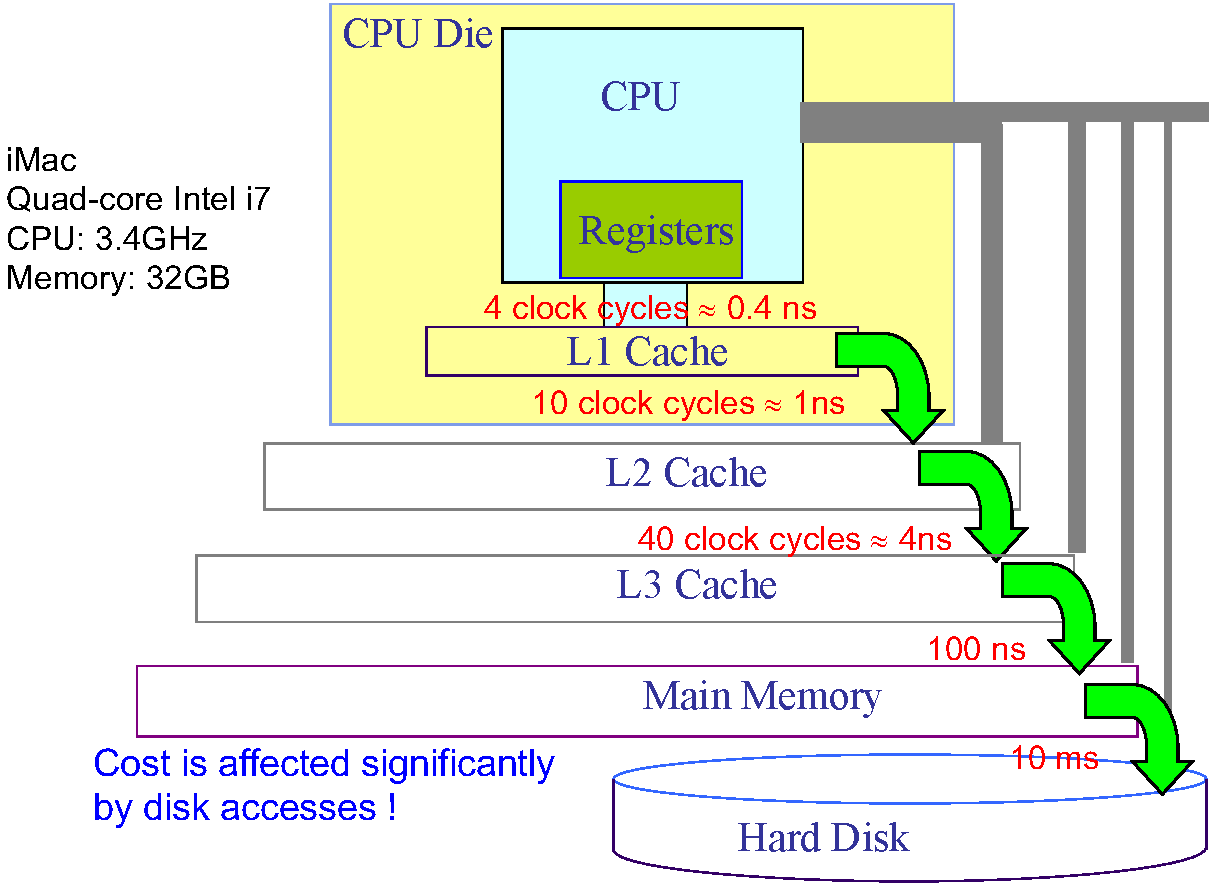
\includegraphics[width=0.6\linewidth]{figs/dbfile-mem-hierarchy.pdf}
    \end{figure}
\end{frame}

\begin{frame}[fragile]
	\frametitle{Design Motivation: The Hard (Magnetic) Disk}
	\begin{figure}
		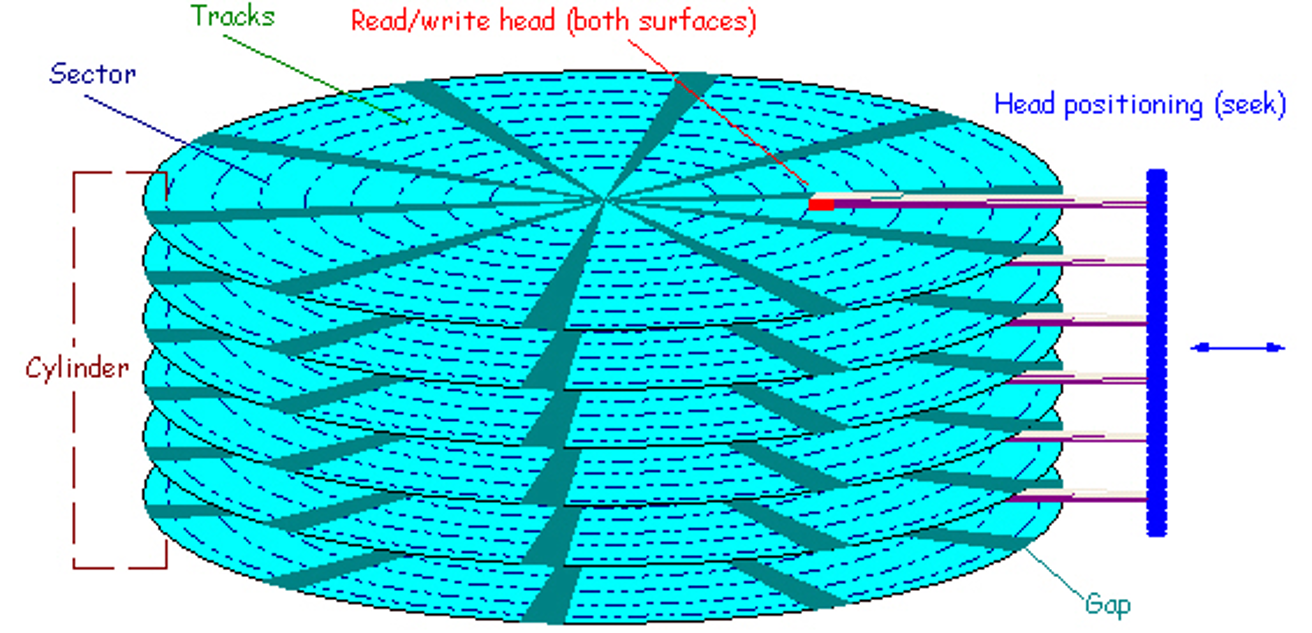
\includegraphics[width=0.5\linewidth]{figs/dbfile-harddisk.png}
	\end{figure}
	\begin{itemize}
		\pause
		\item The time for a \textbf{\emph{disk block access}}, or \textbf{\emph{disk page access}} or 
		\textbf{\emph{disk I/O}}
\\
		\emph{\textcolor{blue}{access time {\rm =} seek time {\rm +} rotational delay {\rm +} transfer time}}
		\pause
		\item Segate Desktop HDD.15: 4TB
		\begin{itemize}
			\item Seek time: 8.5 msec
			\item Rotational delay: 5.1 msec
			\item Transfer rate: 146MB/sec, that is, 0.027msec/4KB
		\end{itemize}
	\end{itemize}
\end{frame}

\begin{frame}[fragile]
	\frametitle{Design Motivation: Storage Hierarchy - Latency}
	\begin{figure}
		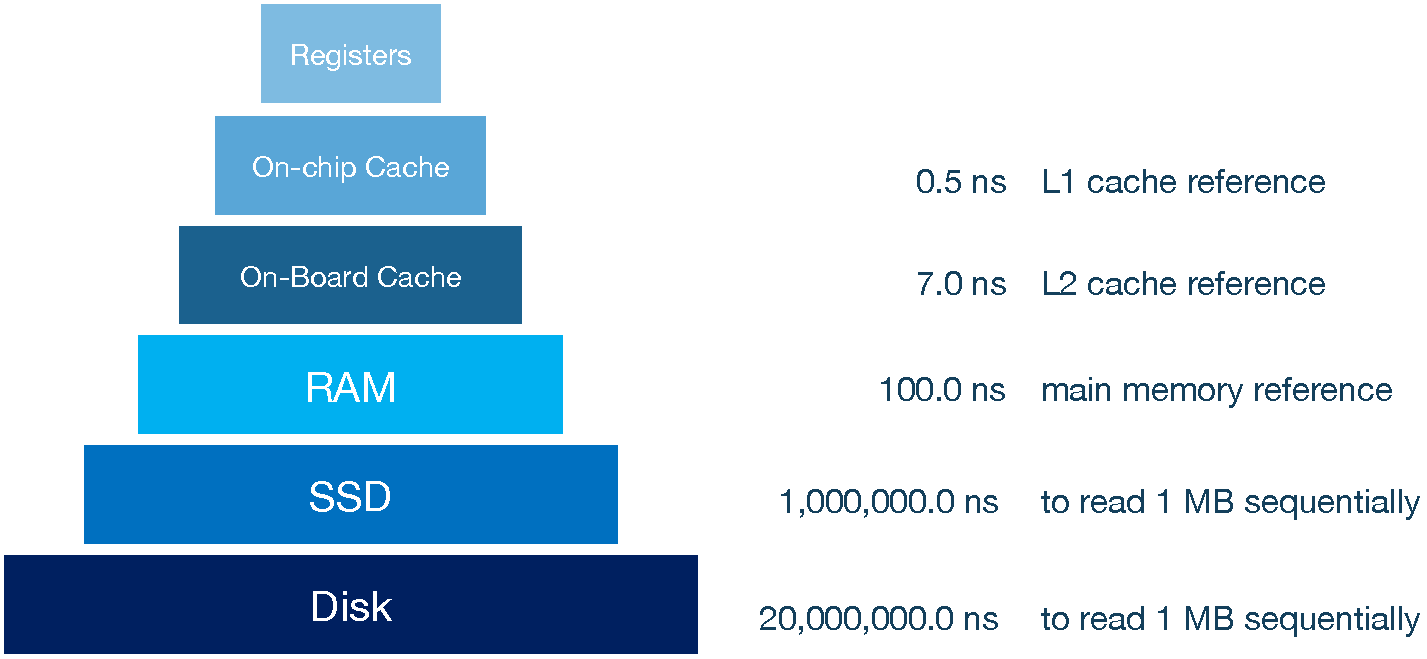
\includegraphics[width=0.85\linewidth]{figs/dbfile-latency1.pdf}
	\end{figure}
\end{frame}

\begin{frame}[fragile]
	\frametitle{Design Motivation: Storage Hierarchy - Latency}
	\begin{figure}
		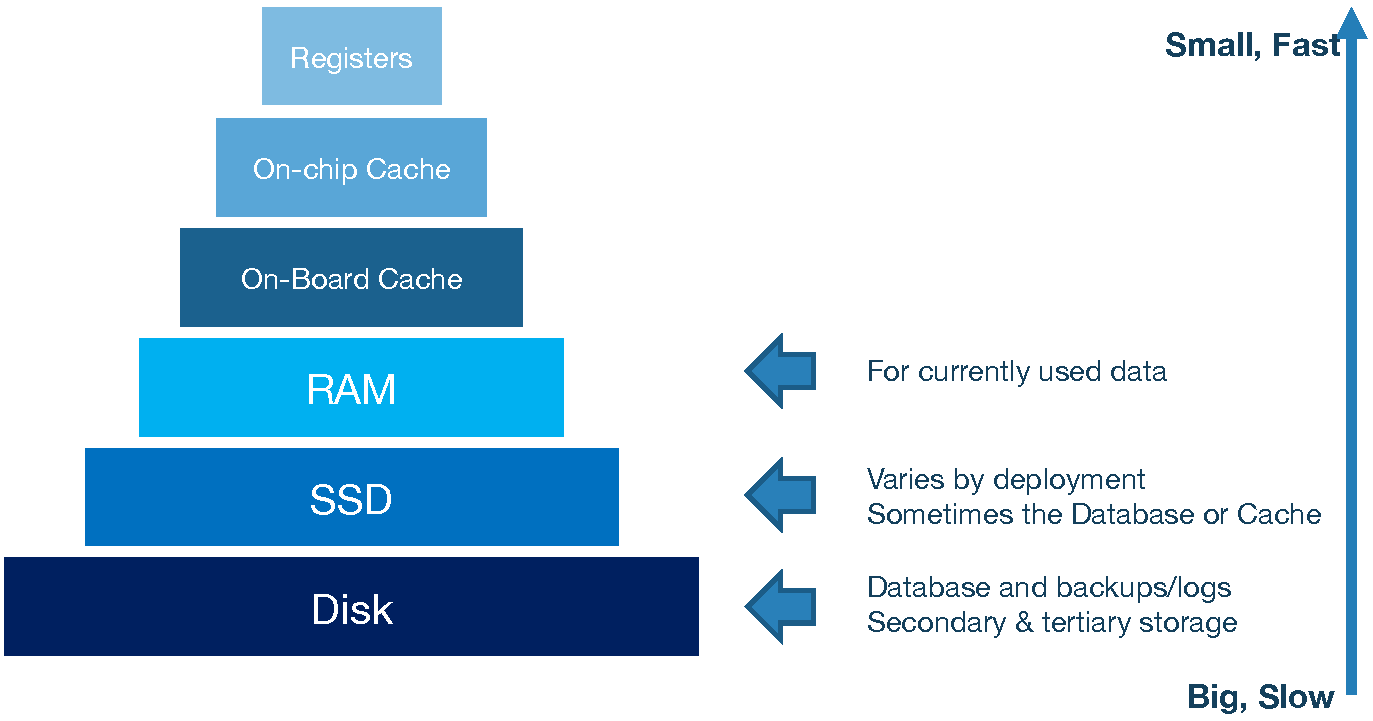
\includegraphics[width=0.85\linewidth]{figs/dbfile-latency2.pdf}
	\end{figure}
\end{frame}



\subsection{DB File: Representations}


\begin{frame}[fragile]
	\frametitle{DB File: Representations}
	\begin{figure}
		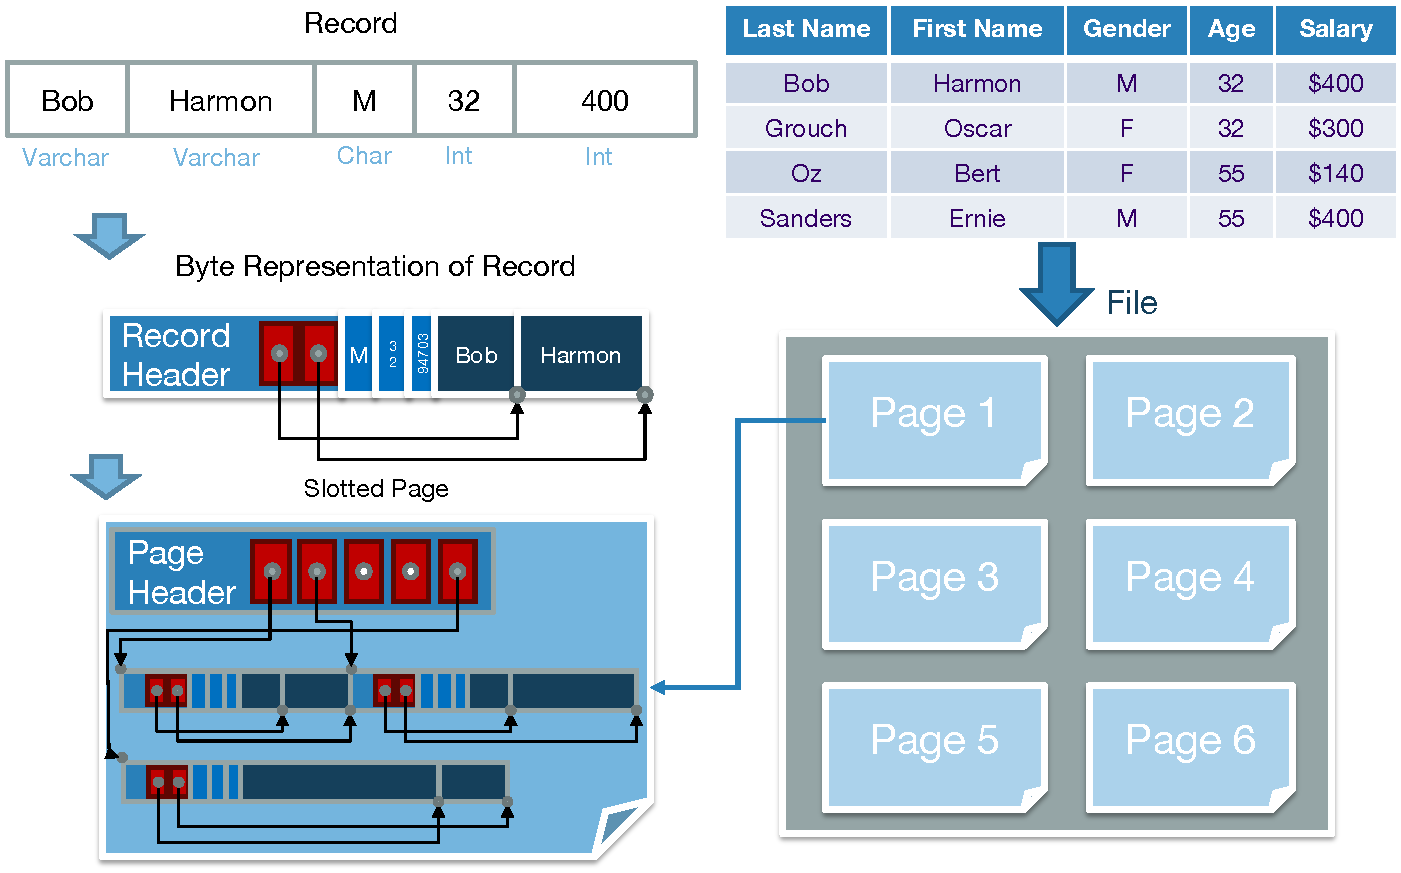
\includegraphics[width=0.75\linewidth]{figs/dbfile-representation.pdf}
	\end{figure}
\end{frame}


\subsection{Page}

\begin{frame}[fragile]
	\frametitle{Page}
	\begin{itemize}
		\item A page is a fixed-size block of data.
		\begin{itemize}
			\item Contain tuples, meta-data, indexes, log records...
			\item Most systems do not mix page types (log/data/index).
			\item Some systems require a page to be self-contained.
		\end{itemize}
		\item Each page is given a unique identifier.
		\begin{itemize}
			\item uses an indirection layer to map pages to physical locations
		\end{itemize}
		\item There are three different notions of "pages" in a DBMS:
		\begin{itemize}
			\item Hardware Page (usually 4KB)
			\item OS Page (usually 4KB)
			\item Database Page (4-16KB)
		\end{itemize}
	\end{itemize}
	\begin{textblock*}{.75\paperwidth}(.46\paperwidth, .55\paperheight) % {block width} (coords)
		\begin{figure}
			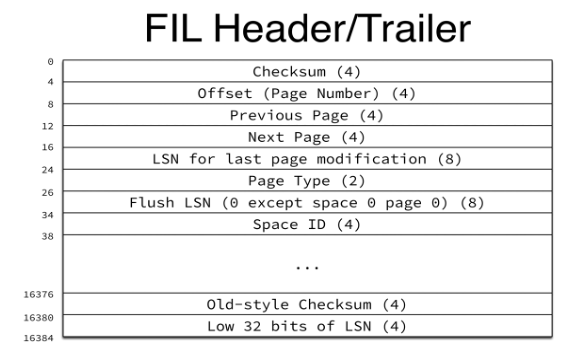
\includegraphics[width=.4\linewidth]{figs/dbfile-fil.png}
		\end{figure}
	\end{textblock*}

\end{frame}


\begin{frame}[fragile]
	\frametitle{Page Header}
	\begin{itemize}
		\item Every page contains a header of meta-data about the page's contents.
		\begin{itemize}
			\item → Page Size
			\item → Checksum
			\item → Transaction Visibility
			\item → Compression Information
		\end{itemize}
		\item Some systems require pages to be self-contained
		\item Design Choice:
		\begin{itemize}
			\item Record length? \textbf{Fixed} or \textbf{Variable}
			\item Find records by record id?
			\item How do we add and delete records?
		\end{itemize}
	\end{itemize}
	\begin{textblock*}{.45\paperwidth}(.52\paperwidth, .3\paperheight) % {block width} (coords)
		\begin{figure}
			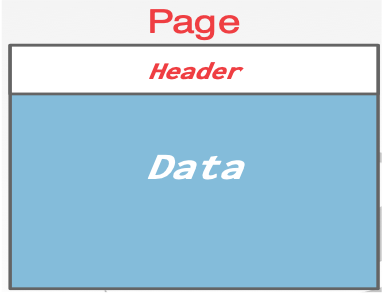
\includegraphics[width=.4\linewidth]{figs/dbfile-pageheader.png}
		\end{figure}
	\end{textblock*}
\end{frame}

\subsection{Page Organization}

\subsubsection{Page Layout}

\begin{frame}[fragile]
	\frametitle{Page Layout}
	\begin{itemize}
		\item Page Layout – disk
		\begin{itemize}
			\item SQLite – 1KB
			\item Oracle/DB2 – 4KB
			\item SQL Server/Postgre – 8KB
			\item MySQL – 16KB
			\item page size, checksum, version
		\end{itemize}
		\item Record Layout
	\end{itemize}
	\begin{textblock*}{.9\paperwidth}(.25\paperwidth, .1\paperheight) % {block width} (coords)
		\begin{figure}
			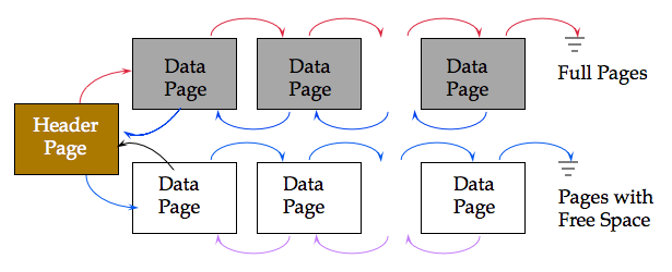
\includegraphics[width=.4\linewidth]{figs/dbfile-heapfile1.png}
		\end{figure}
	\end{textblock*}
	\begin{textblock*}{.9\paperwidth}(.25\paperwidth, .35\paperheight) % {block width} (coords)
		\begin{figure}
			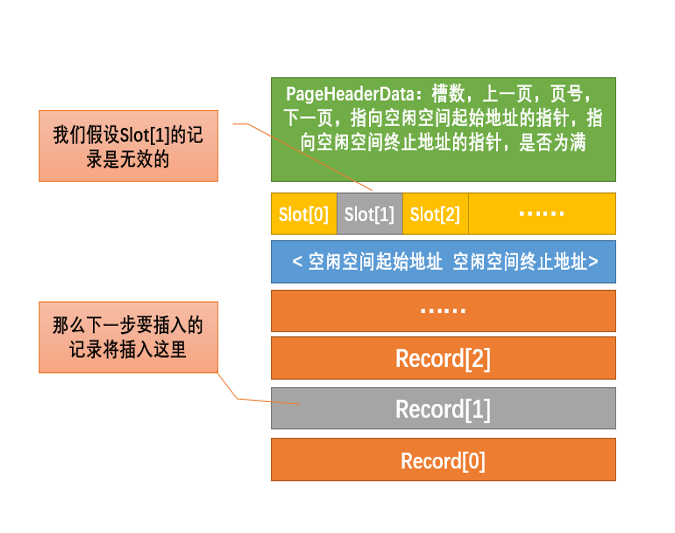
\includegraphics[width=.4\linewidth]{figs/dbfile-records.png}
		\end{figure}
	\end{textblock*}
\end{frame}


\begin{frame}[fragile]
	\frametitle{Heap File Implemented as List}
	\begin{figure}
		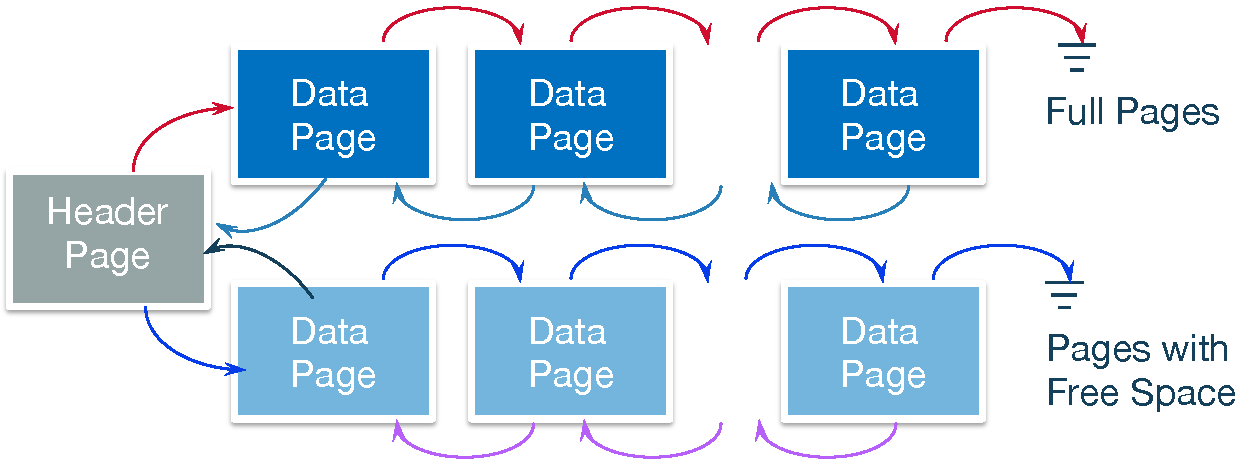
\includegraphics[width=.7\linewidth]{figs/dbfile-heapfile2.pdf}
	\end{figure}
	\begin{itemize}
		\item Header page ID and Heap file name stored elsewhere
		\begin{itemize}
			\item Database catalog
		\end{itemize}
		\item Each page contains 2 "pointers" plus \textbf{free space} and \textbf{data}
		\item What is wrong with this?
		\begin{itemize}
			\item How do I find a page with enough space for a 20 byte record?
		\end{itemize}
	\end{itemize}
\end{frame}

\subsubsection{Page Directory}

\begin{frame}[fragile]
	\frametitle{Page Directory}
	\begin{figure}
		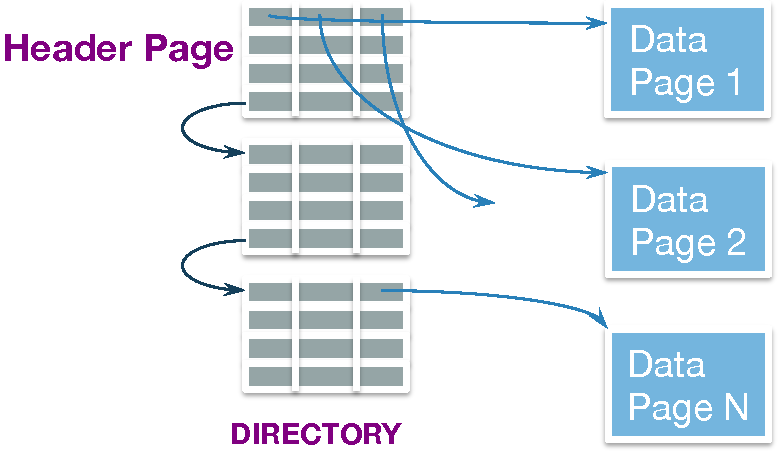
\includegraphics[width=.45\linewidth]{figs/dbfile-page-directory.pdf}
	\end{figure}
	\begin{itemize}
		\item Directory entries include \#free bytes on the referenced page
		\item Header pages accessed often → likely in cache
		\item Finding a page to fit a record required far fewer page loads than linked list (Why?)
		\begin{itemize}
			\item One header page load reveals free space of many pages
		\end{itemize}
	\end{itemize}
\end{frame}

\begin{frame}[fragile]
	\frametitle{Page Organizations}
	
	\textbf{Many alternatives exist, each good in some situations and not so good in others. 
		(This is a theme in DB systems work!)}
	
	\begin{itemize}
		\item \textbf{Heap Files}: Suitable when typical access is a \textcolor{blue}{full scan} of all records
		\item \textbf{Sorted Files}: Best for retrieval in \textcolor{blue}{order}, 
		or when a \textcolor{blue}{range} of records is needed
		\item \textbf{Hashing Files}: Using a hash to organize the pages
		\item \textbf{Clustered Files \& Indexes}: 
			Group data into blocks to enable fast \textcolor{blue}{lookup} and efficient 
			\textcolor{blue}{modifications}.
	\end{itemize}
\end{frame}

\begin{frame}[fragile]
	\frametitle{Page Layout}
	DBMSs manage pages in files on disk in different ways.
	\begin{figure}
		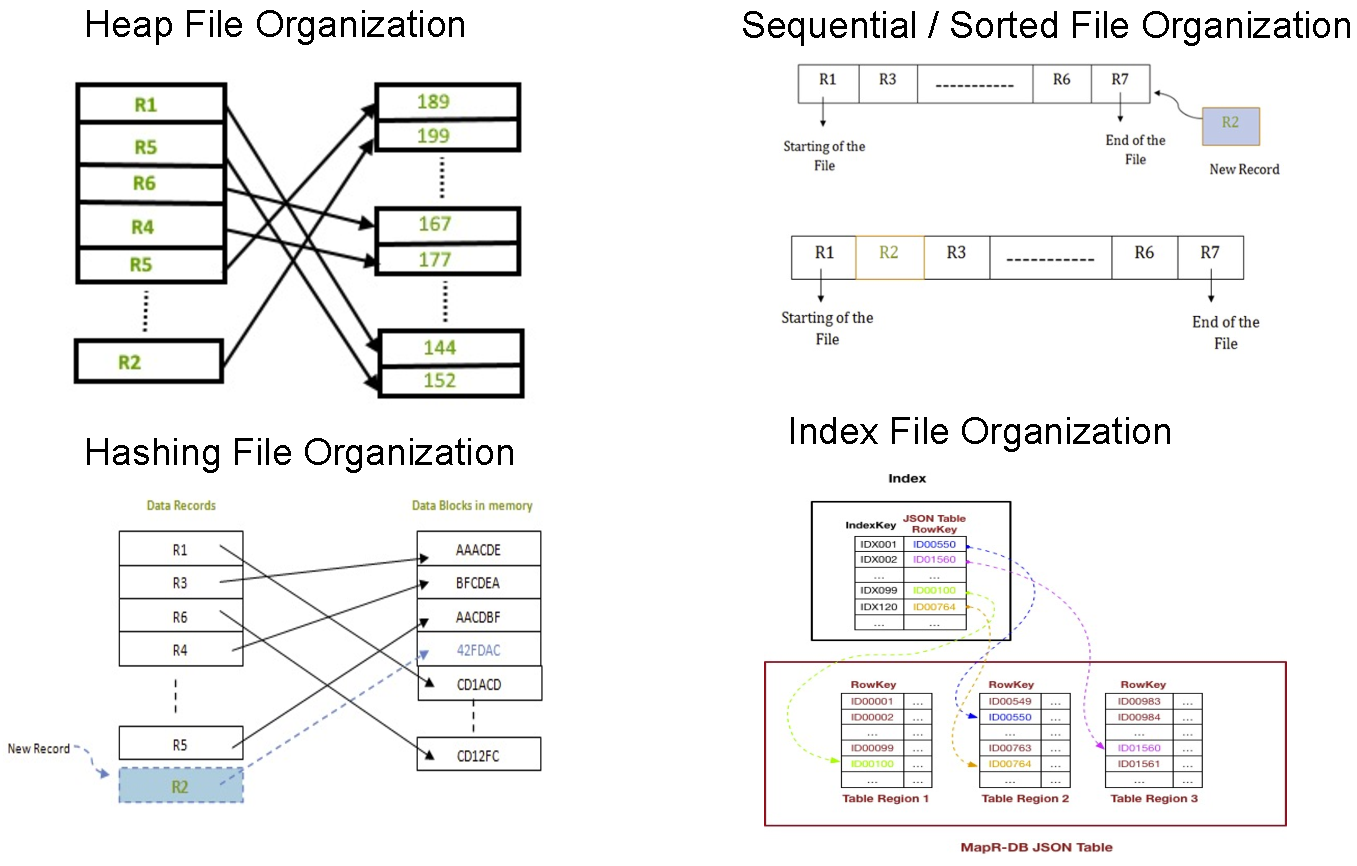
\includegraphics[width=.7\linewidth]{figs/dbfile-layouts.pdf}
	\end{figure}
\end{frame}


\begin{frame}[fragile]
	\frametitle{Table, Segment, Page}
	\begin{figure}
		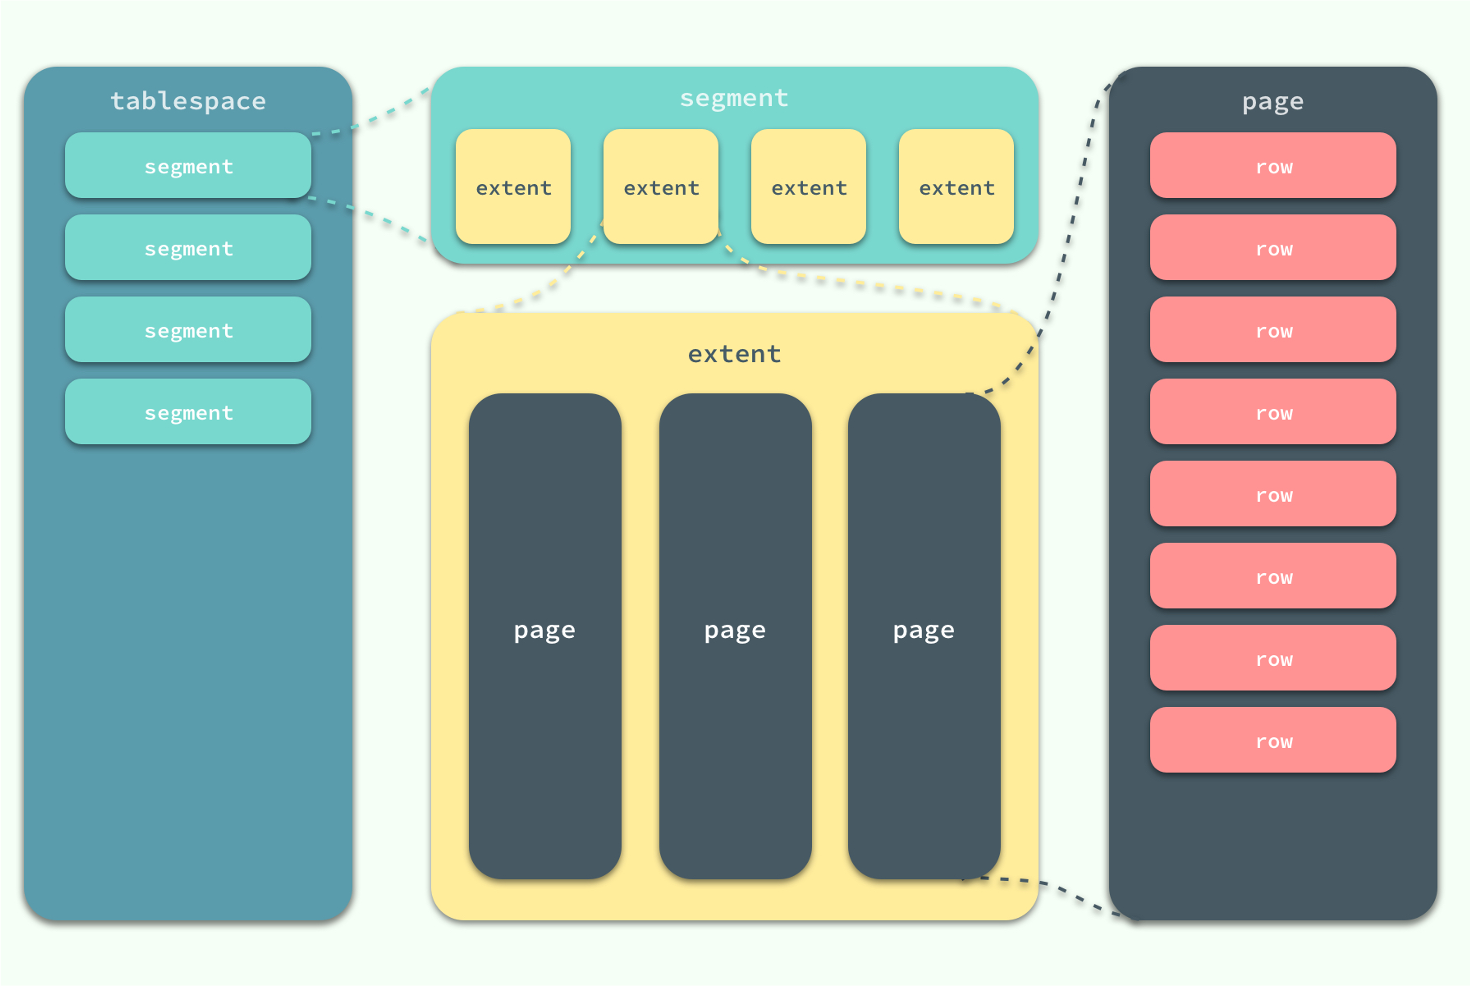
\includegraphics[width=.68\linewidth]{figs/dbfile-table-seg-page1.png}
	\end{figure}
\end{frame}

\begin{frame}[fragile]
	\frametitle{Table, Segment, Page}
	\begin{figure}
		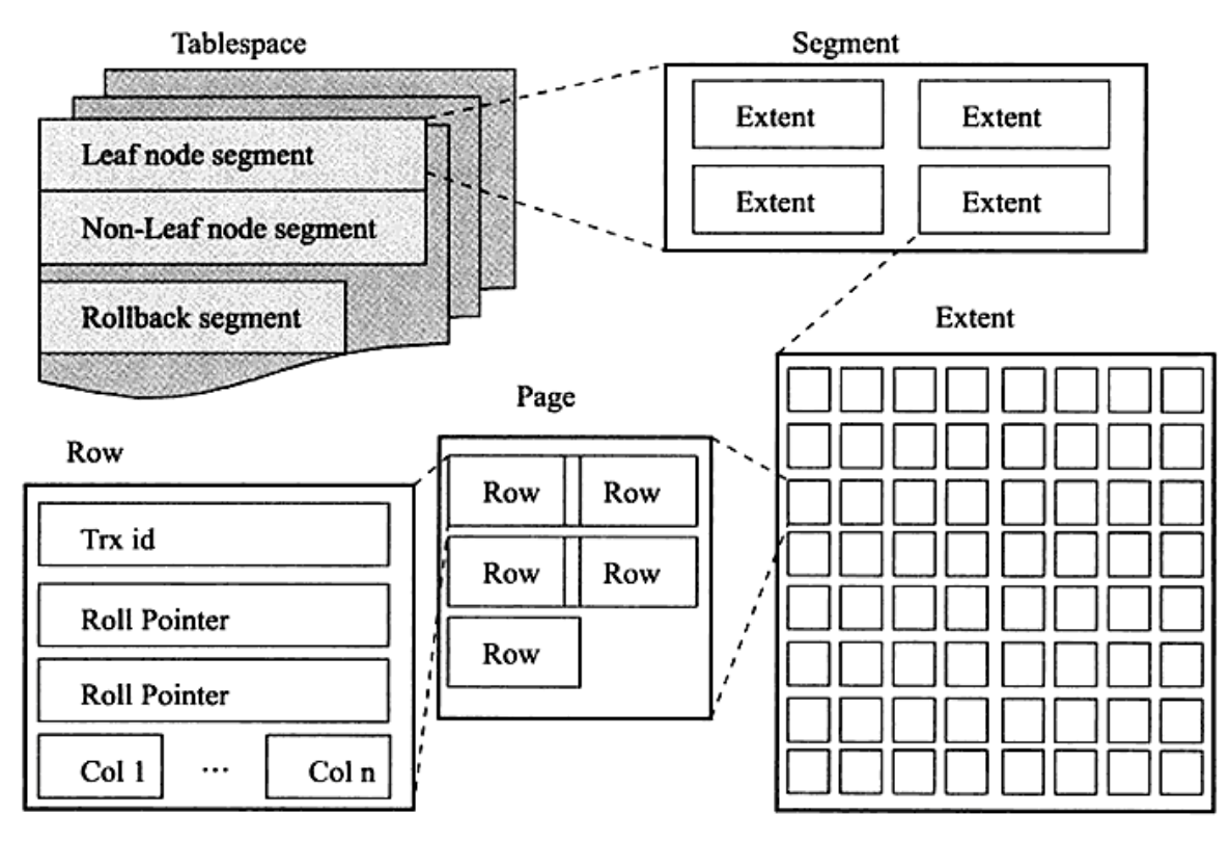
\includegraphics[width=.68\linewidth]{figs/dbfile-table-seg-page2.png}
	\end{figure}
\end{frame}


\begin{frame}[fragile]
	\frametitle{Page Summary}
	\begin{figure}
		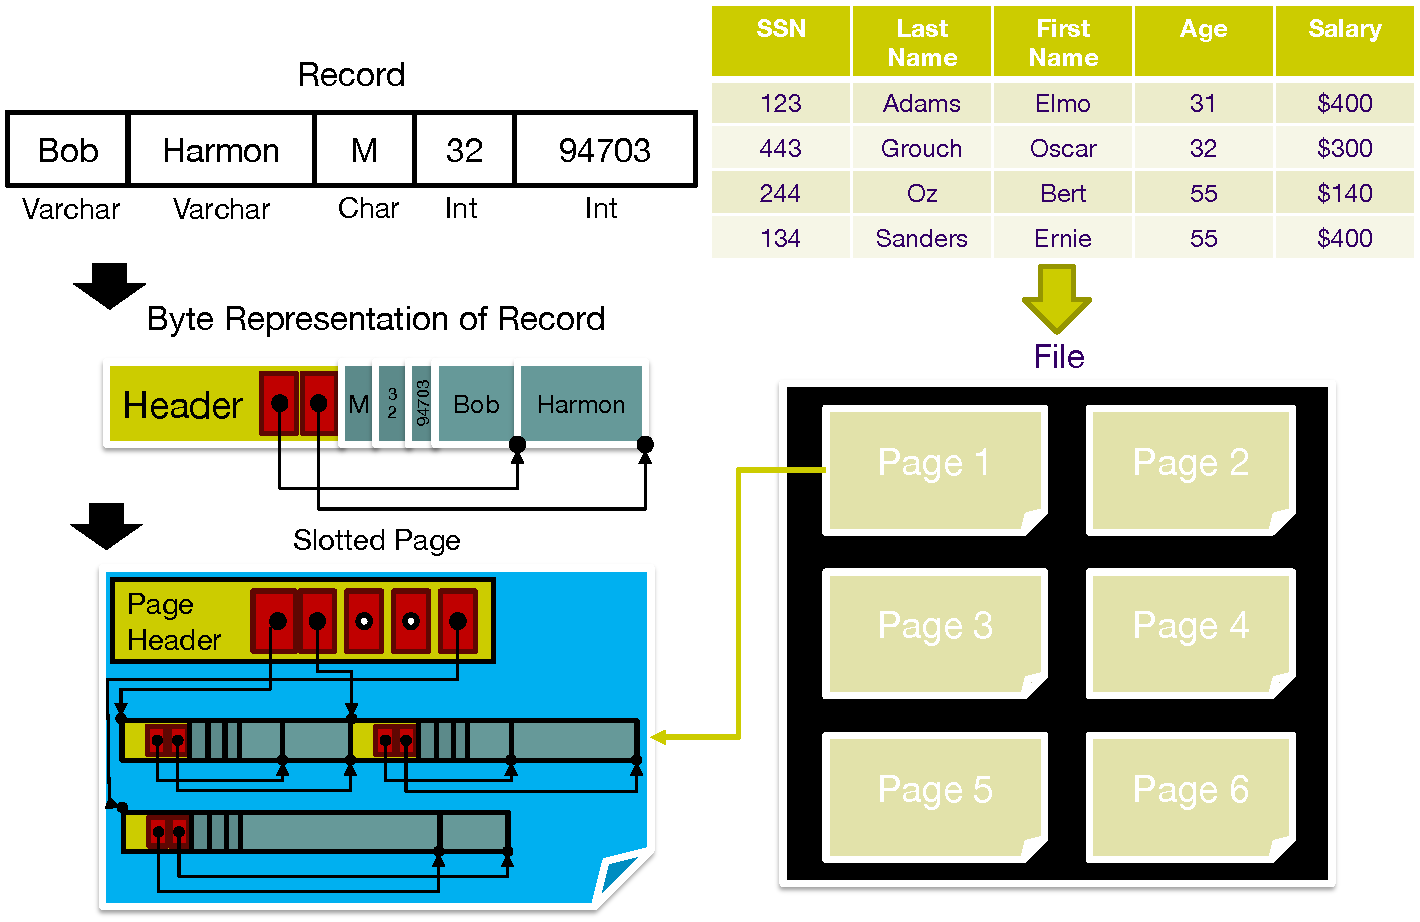
\includegraphics[width=.68\linewidth]{figs/dbfile-page-summary.pdf}
	\end{figure}
\end{frame}


\subsection{Page Persistence}

\subsubsection{Two Questions}

\begin{frame}[fragile]
	\frametitle{Q1: Dirty Pages}
	\begin{figure}
		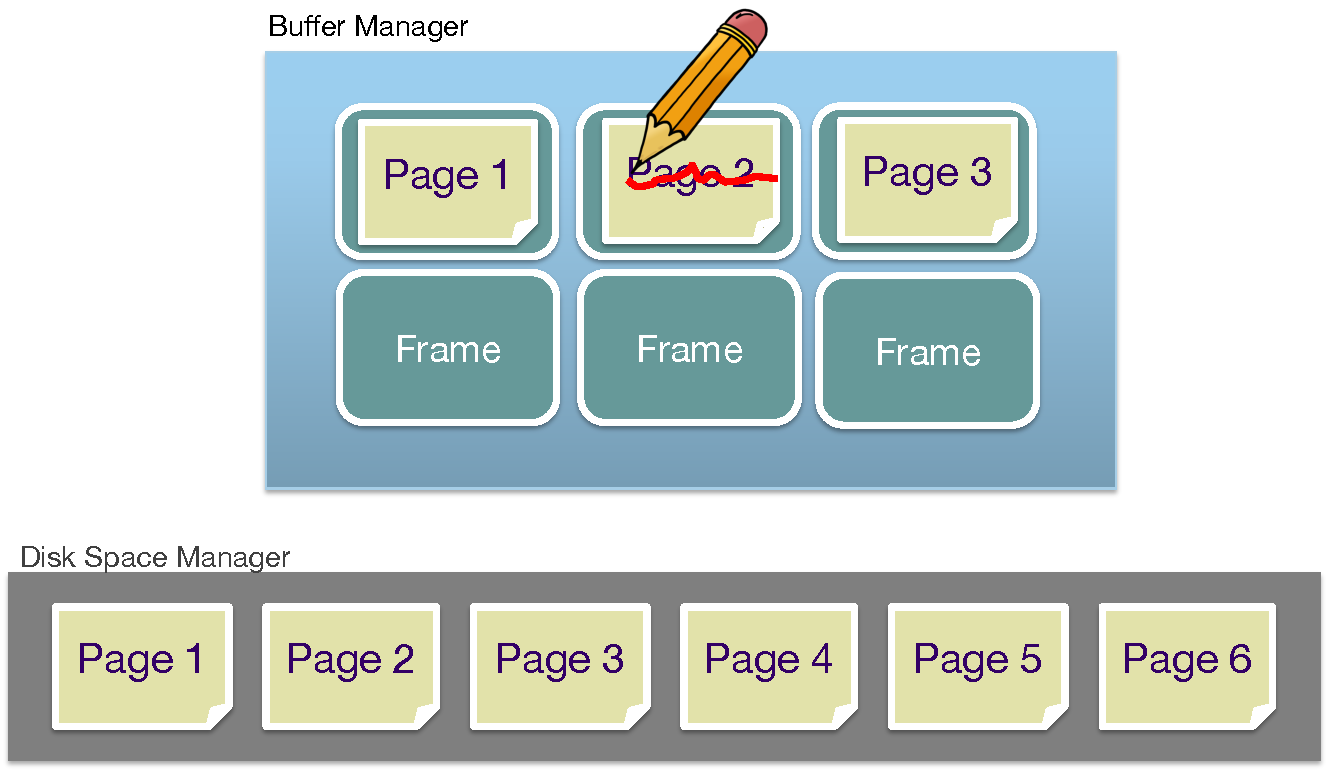
\includegraphics[width=.68\linewidth]{figs/dbfile-dirtypage.pdf}
	\end{figure}
\end{frame}

\begin{frame}[fragile]
	\frametitle{Q2: Page Replacement}
	\begin{figure}
		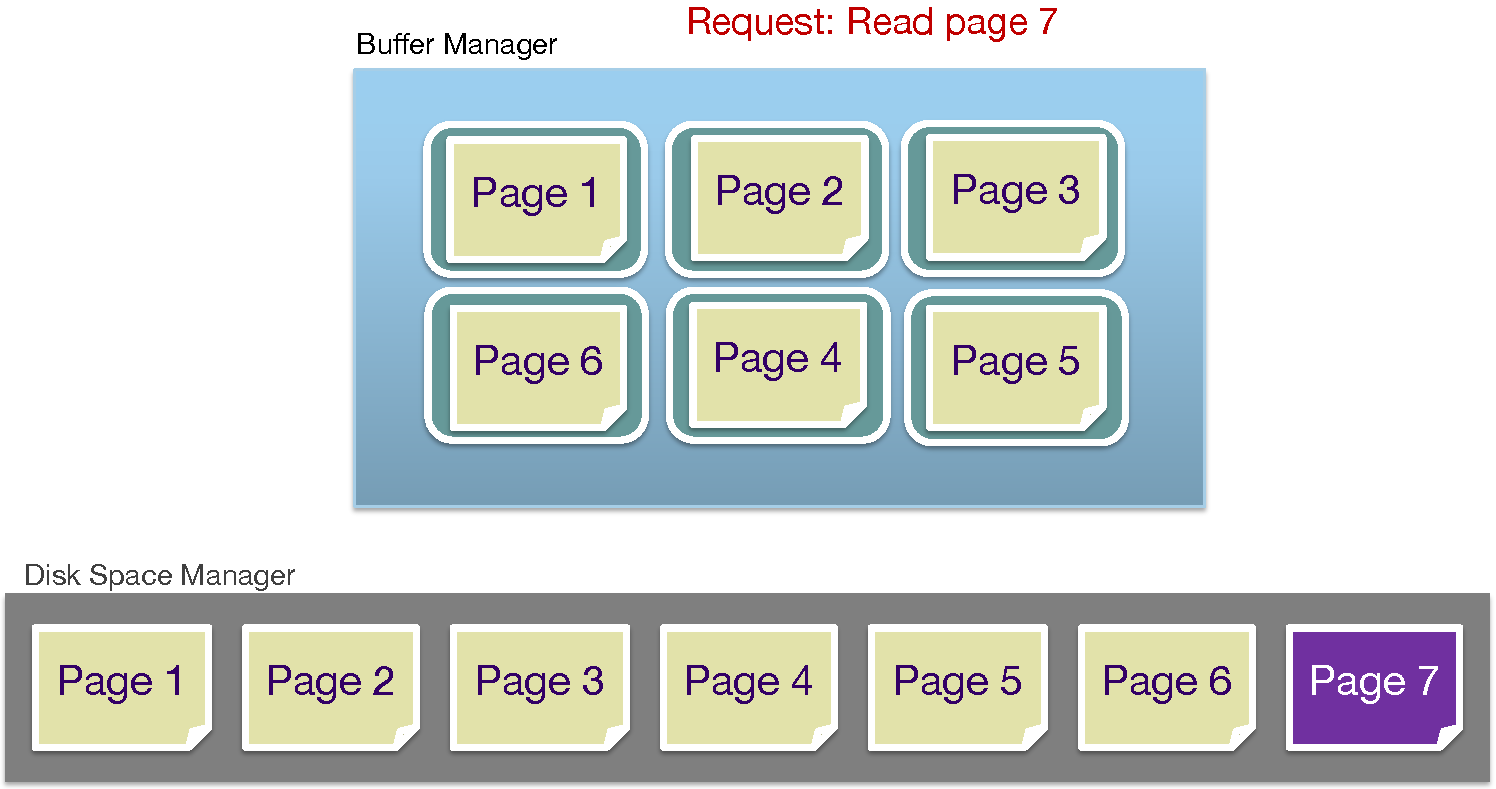
\includegraphics[width=.68\linewidth]{figs/dbfile-replacement.pdf}
	\end{figure}
\end{frame}

\begin{frame}[fragile]
	\frametitle{Questions We Need to Answer}
	\begin{itemize}
		\item Handling dirty pages
		\begin{itemize}
			\item How will the buffer manager find out?
			\begin{itemize}
				\item \emph{Dirty bit} on page
			\end{itemize}
			\item What to do with a dirty page?
			\begin{itemize}
				\item \emph{Write back} via disk manager
			\end{itemize}
		\end{itemize}
		\item Page Replacement
		\begin{itemize}
			\item How will the buffer mgr know if a page is “in use”?
			\begin{itemize}
				\item Page \emph{pin count}
			\end{itemize}
			\item If buffer manager is full, what page should be replaced?
			\begin{itemize}
				\item Page \emph{replacement policy}
			\end{itemize}
		\end{itemize}
	\end{itemize}
\end{frame}

\subsubsection{Write-Ahead Log}

\begin{frame}[fragile]
	\frametitle{Log}
	\begin{itemize}
		\item Why log?
		\begin{itemize}
			\item A sequence of data updates
			\item Random access to sequential access
			\item Recovery
		\end{itemize}
	\end{itemize}
	\begin{figure}
		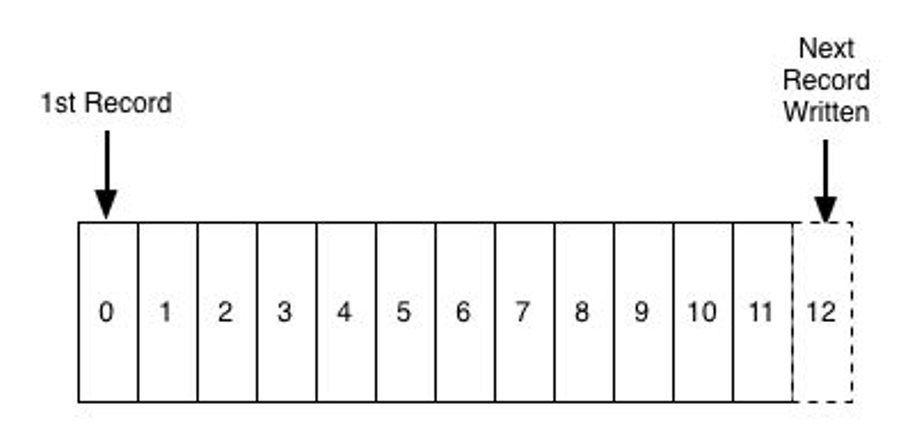
\includegraphics[width=.65\linewidth]{figs/dbfile-log.png}
	\end{figure}
\end{frame}

\begin{frame}[fragile]
	\frametitle{Write-Ahead Log}
	\begin{itemize}
		\item Random write → Sequential write
	\end{itemize}
	\begin{figure}
		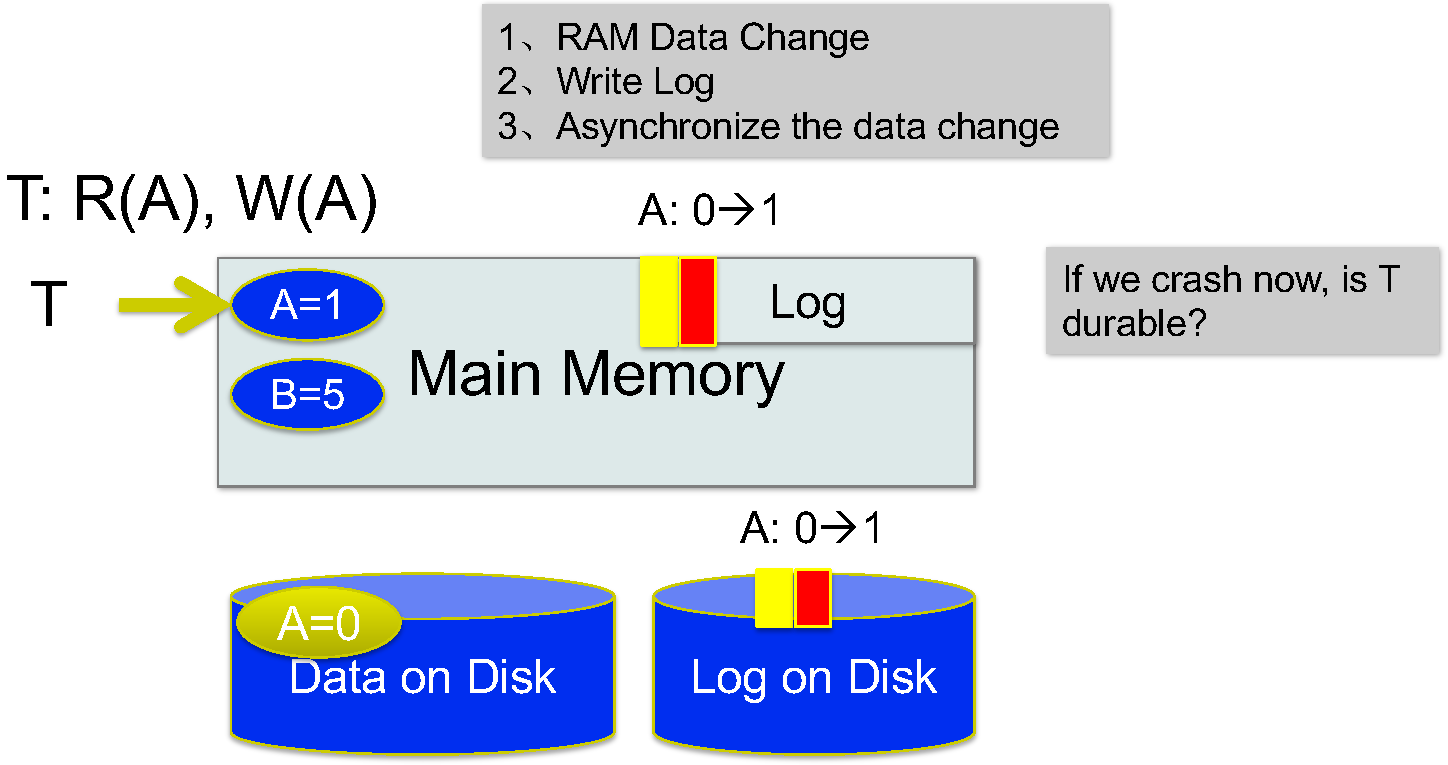
\includegraphics[width=.68\linewidth]{figs/dbfile-wal1.pdf}
	\end{figure}
\end{frame}

\begin{frame}[fragile]
	\frametitle{Write-Ahead Log}
	\begin{itemize}
		\item Random write → Sequential write
	\end{itemize}
	\begin{figure}
		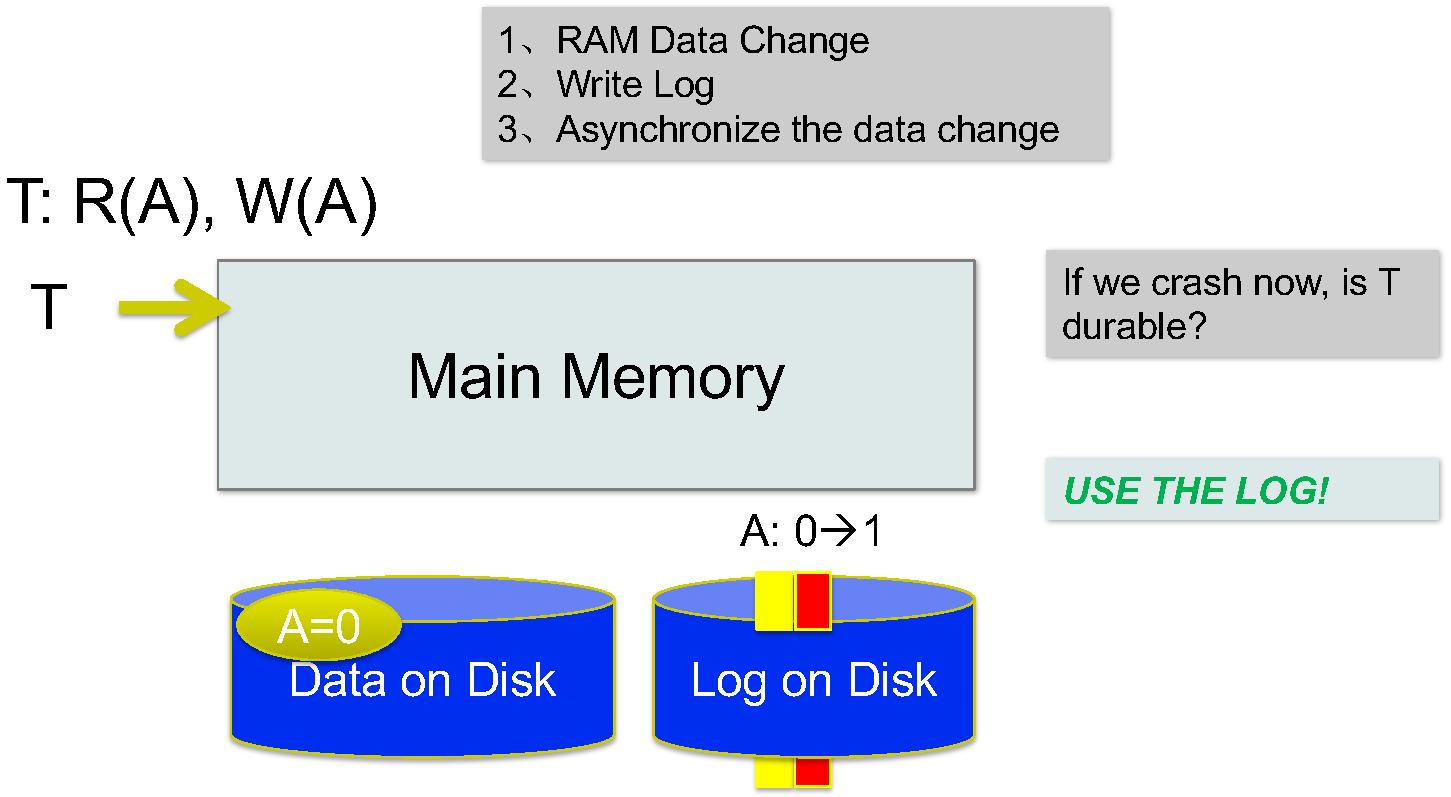
\includegraphics[width=.68\linewidth]{figs/dbfile-wal2.pdf}
	\end{figure}
\end{frame}

\begin{frame}[fragile]
	\frametitle{Write-Ahead Log}
	\begin{itemize}
		\item Random write → Sequential write
	\end{itemize}
	\begin{figure}
		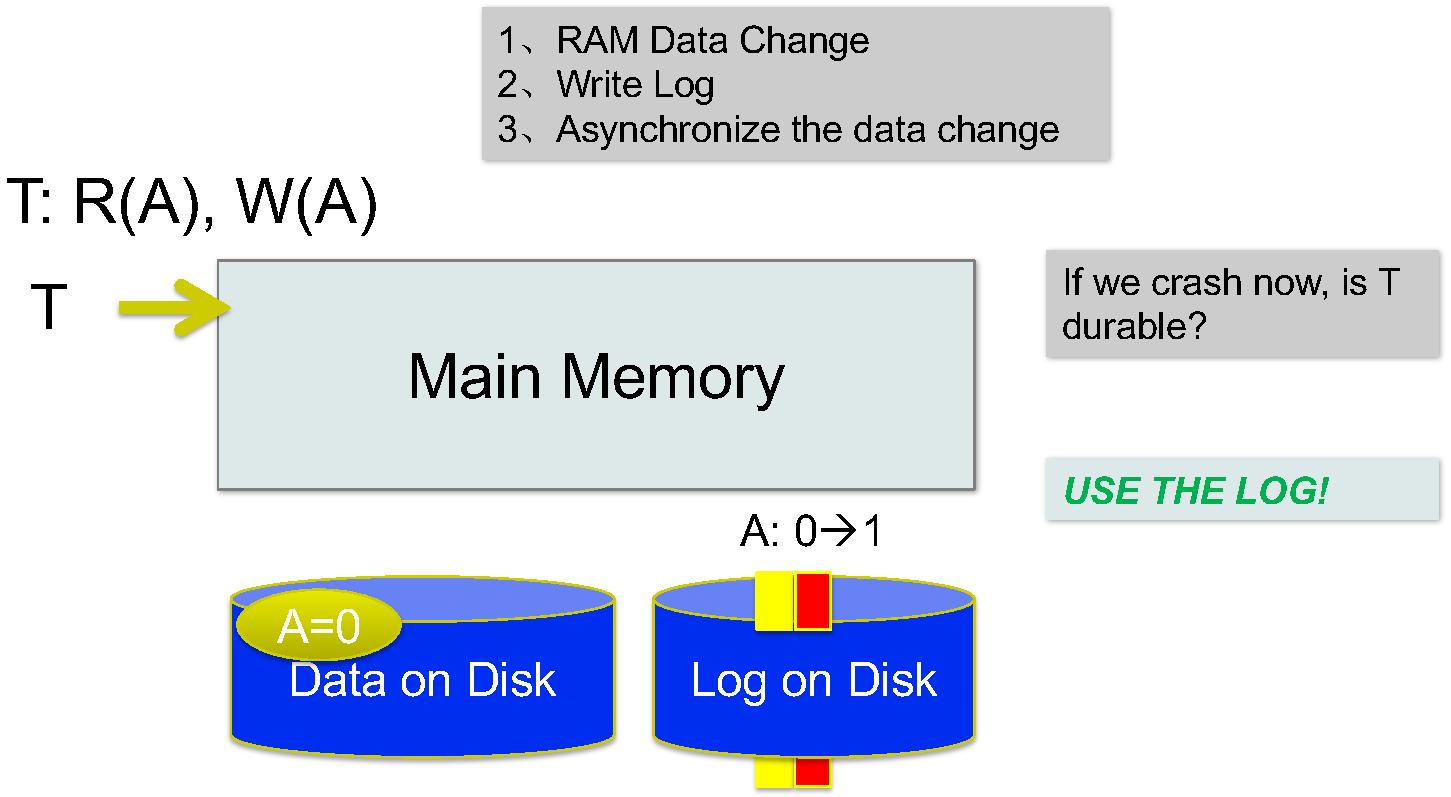
\includegraphics[width=.68\linewidth]{figs/dbfile-wal2.pdf}
	\end{figure}
\end{frame}

\begin{frame}[fragile]
	\frametitle{Log}
	\begin{textblock*}{.75\paperwidth}(.35\paperwidth, .1\paperheight) % {block width} (coords)
		\begin{figure}
			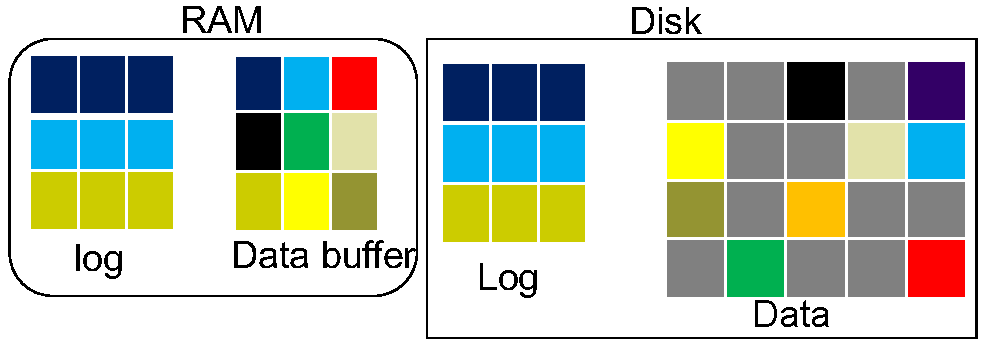
\includegraphics[width=.7\linewidth]{figs/dbfile-log2.pdf}
		\end{figure}
	\end{textblock*}
	\begin{textblock*}{.75\paperwidth}(.35\paperwidth, .45\paperheight) % {block width} (coords)
		\begin{figure}
			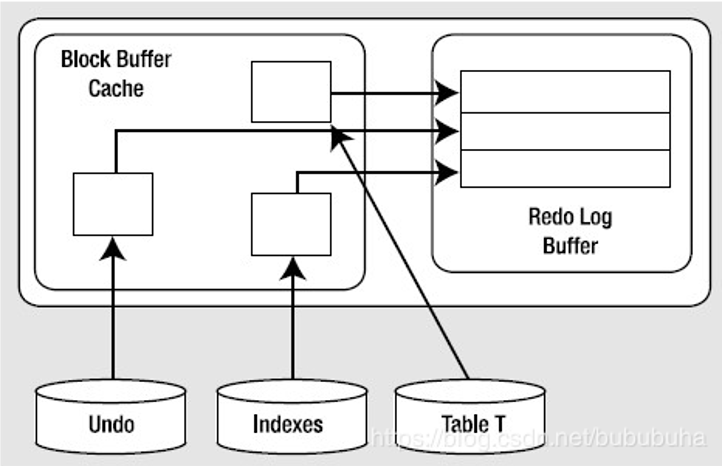
\includegraphics[width=.45\linewidth]{figs/dbfile-log3.png}
		\end{figure}
	\end{textblock*}
	\begin{itemize}
		\item Log
		\begin{itemize}
			\item Random → Sequential
			\item Recovery
		\end{itemize}
		\pause
		~\\
		\noindent Factors
		\item Recovery
		\begin{itemize}
			\item Transaction Failures
			\item System Failures
			\item Hardware Failures
		\end{itemize}
		\item Low Latency
		\item High Throughput
	\end{itemize}
\end{frame}

\subsection{High Availability}

\begin{frame}[fragile]
	\frametitle{High Availability}
	\begin{itemize}
		\item 一主一备
		\begin{figure}
			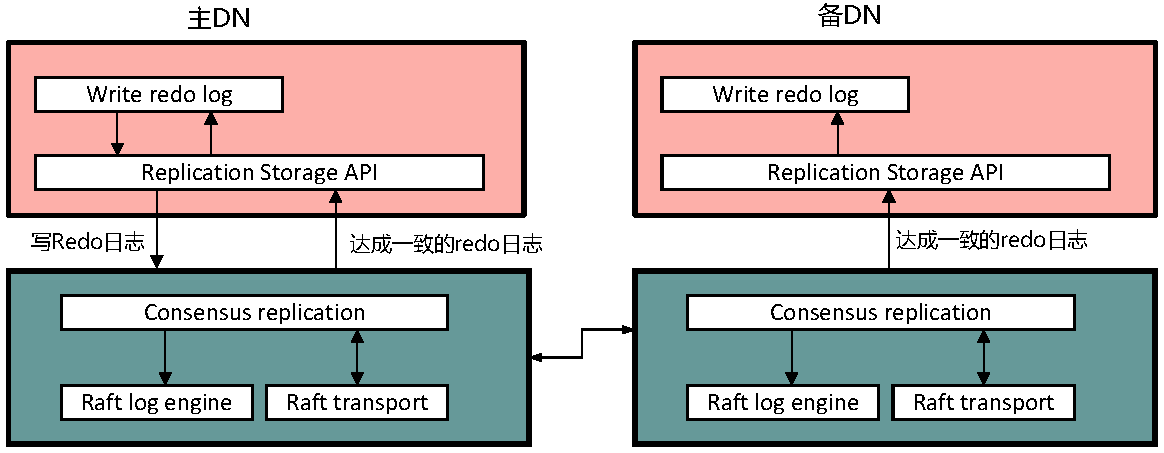
\includegraphics[width=.7\linewidth]{figs/dbfile-ha.pdf}
		\end{figure}
		\item 一主多备
		\begin{itemize}
			\item Paxos:多数派
			\item Quorum:R+W>N; R: 读节点数,W:写节点数,N:总节点数
		\end{itemize}
	\end{itemize}
\end{frame}

%----------------------------------------------
% ##### Built-in Compression
% 
% Ref: http://pages.cs.wisc.edu/~remzi/OSTEP/Citations/zfs_last.pdf Page 29
% 
% %% figure
% 	\begin{figure}
% 	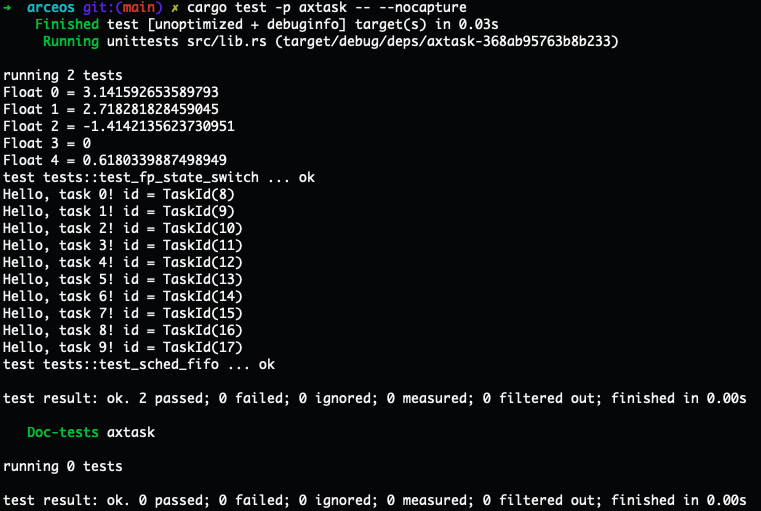
\includegraphics[width=0.8\linewidth]{test}
% %	\caption{xxxx}
% 	\end{figure}
% ![ZFS-compression](figs/ZFS-compression.png)
% 
% %% itemize
%     \begin{itemize}
%         \item xx
%     \end{itemize}
%  * Block-level compression in SPA
%  * Transparent to all other layers
%  * Each block compressed independently
%  * All-zero blocks converted into file holes
%  * LZJB and GZIP available today; more on the way
%----------------------------------------------
\end{document}
